\chapter{Практическая часть}
\section{Код программы}
Модуль разработанных алгоритмов представлен на листинге \ref{lst:code}
\begin{lstlisting}[label=lst:code, caption=Модуль разработанных алгоритмов, basicstyle=\footnotesize]
##Тартыков Лев ИУ7-64Б, 2022 г
pkg load statistics;
clc;
clear all;

function main()
	[error_read_file, x] = load_data("data.txt");
	if (error_read_file != 0)
		return;
	endif   
	gamma = input_gamma();
	find_parametres(x, gamma);
	plot_graphs(x, gamma);
endfunction

function [error, x] = load_data(file_name)
	x = []; i = 1; error = 0;
	file = fopen(file_name, "r");
	if (file == -1)
		error = -1;
	else
		end_file = 0;
		while (end_file == 0)
			if (feof(file))
				end_file = 1;
			else
				x(i) = fscanf(file, '%f', [1,1]);
				fscanf(file, '%c', [1, 1]);
				i++;
			endif
		endwhile
	endif
	fclose(file);
endfunction

function [gamma] = input_gamma()
	gamma = input('Введите значение уровня доверия: ');    
endfunction

function find_parametres(x, gamma)
	alpha = (1 + gamma) / 2;
	count_x = length(x);
	mu = find_mu(x, count_x)
	S_2 = find_S_2(x, mu, count_x)
	
	mu_low = find_mu_low(mu, sqrt(S_2), count_x, alpha)
	mu_high = find_mu_high(mu, sqrt(S_2), count_x, alpha)
	
	sigma_2_low = find_DX_low(S_2, count_x, alpha)
	sigma_2_high = find_DX_high(S_2, count_x, alpha)
endfunction

function plot_graphs(x, gamma)
	count_x = length(x); alpha = (1 + gamma) / 2;
	mu_array = []; mu_low_array = []; mu_high = [];
	sigma_2_array = []; sigma_2_low_array = []; sigma_2_high_array = [];
	
	for i = 1: count_x
		mu = find_mu(x(1:i), i);
		S_2 = find_S_2(x(1:i), mu, i);
		
		mu_array(i) = mu;
		sigma_2_array(i) = S_2;
		mu_low_array(i) = find_mu_low(mu, sqrt(S_2), i, alpha);
		mu_high_array(i) = find_mu_high(mu, sqrt(S_2), i, alpha);
		
		sigma_2_low_array(i) = find_DX_low(S_2, i, alpha);
		sigma_2_high_array(i) = find_DX_high(S_2, i, alpha);
	endfor
	
	mu = find_mu(x, count_x);
	S_2 = find_S_2(x, mu, count_x);
	
	figure
	subplot(1, 2, 1);
	hold on;
	plot([1,count_x], [mu, mu]);
	plot((1:count_x), mu_array);
	plot((1:count_x), mu_low_array);
	plot((1:count_x), mu_high_array);
	xlabel('n');
	ylabel('y');
	legend('mu(x_N)','mu(x_n)','mu_low(xn)','mu_high(xn)');
	hold off;
	
	subplot(1, 2, 2);
	hold on;
	plot((1:count_x), (zeros(1, count_x) + S_2));
	plot((1:count_x), sigma_2_array);
	plot((1:count_x), sigma_2_low_array);
	plot((1:count_x), sigma_2_high_array);
	xlabel('n');
	ylabel('z');
	legend('S_2(x_N)','S_2(x_n)','sigma_low(xn)','sigma_high(xn)');
	hold off;

endfunction

function [mu] = find_mu(x, count_x)
	mu = sum(x) / count_x;
endfunction

function [S_2] = find_S_2(x, mu, count_x)
	S_2 = sum((x - mu).^2) / (count_x - 1);
endfunction

function [mu_low] = find_mu_low(avg_x, S, n, alpha)
	mu_low = avg_x - tinv(alpha, n-1) * S / sqrt(n);
endfunction

function [mu_high] = find_mu_high(avg_x, S, n, alpha)
	mu_high = avg_x + tinv(alpha, n-1) * S / sqrt(n);
endfunction

function [sigma_2_low] = find_DX_low(S_2, n, alpha)
	sigma_2_low = S_2 * (n - 1) / chi2inv(1 - alpha, n-1); 
endfunction

function [sigma_2_high] = find_DX_high(S_2, n, alpha)
	sigma_2_high = S_2 * (n - 1) / chi2inv(alpha, n-1); 
endfunction

main();
\end{lstlisting}

\newpage
\section{Результаты расчетов для выборки из индивидуального варианта (при построении графиков принять $\gamma$ = 0.9).}
Согласно варианту 15, результаты расчетов для выборки приведены в формулах (\ref{eq:res_mu}), (\ref{eq:res_s_2}), (\ref{eq:mu_low}), (\ref{eq:mu_high}), (\ref{eq:sigma_2_low}), (\ref{eq:sigma_2_high}).
\begin{equation}
	\label{eq:res_mu}
	\hat\mu(\vec x_n) = -3.6762
\end{equation}
\begin{equation}
	\label{eq:res_s_2}
	S^2(\vec{x_n}) = 0.8664
\end{equation}
\begin{equation}
	\label{eq:mu_low}
	\underline\mu(\vec x_n) = -3.8170
\end{equation}
\begin{equation}
	\label{eq:mu_high}
	\overline\mu(\vec x_n) = -3.5353
\end{equation}
\begin{equation}
	\label{eq:sigma_2_low}
	\underline\sigma^2(\vec x_n) = 1.0875
\end{equation}
\begin{equation}
	\label{eq:sigma_2_high}
	\overline\sigma^2(\vec x_n) = 0.7088
\end{equation}

На рисунке \ref{image:graph1} представлены график прямой $y = \hat\mu(\vec x_N)$ и функций \newline $y = \hat\mu(\vec x_n),\ y = \underline\mu(\vec x_n),\  y = \overline\mu(\vec x_n)$ как функции объема n выборки, где n изменяется от 1 до N.
\begin{figure}[H]
	\centering{
		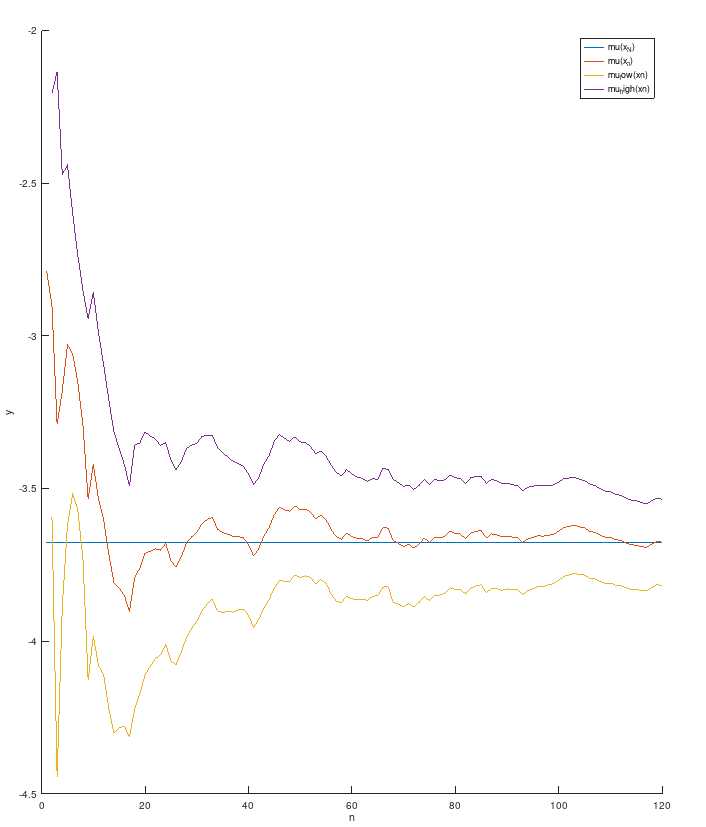
\includegraphics[scale=0.5]{./images/graph_1}
		\caption{График прямой $y=\hat\mu(\vec x_N)$ и функций $y=\hat\mu(\vec x_n),\ y=\underline\mu(\vec x_n),\  y=\overline\mu(\vec x_n)$ как функции объема n выборки.}
		\label{image:graph1}
	}
\end{figure}

На рисунке \ref{image:graph1} представлены график прямой $z=S^2(\vec x_N)$ и функций \newline $z=S^2(\vec x_n),\ z=\underline\sigma^2(\vec x_n),\  z=\overline\sigma^2(\vec x_n)$ как функции объема n выборки, где n изменяется от 1 до N.
\begin{figure}[H]
	\centering{
		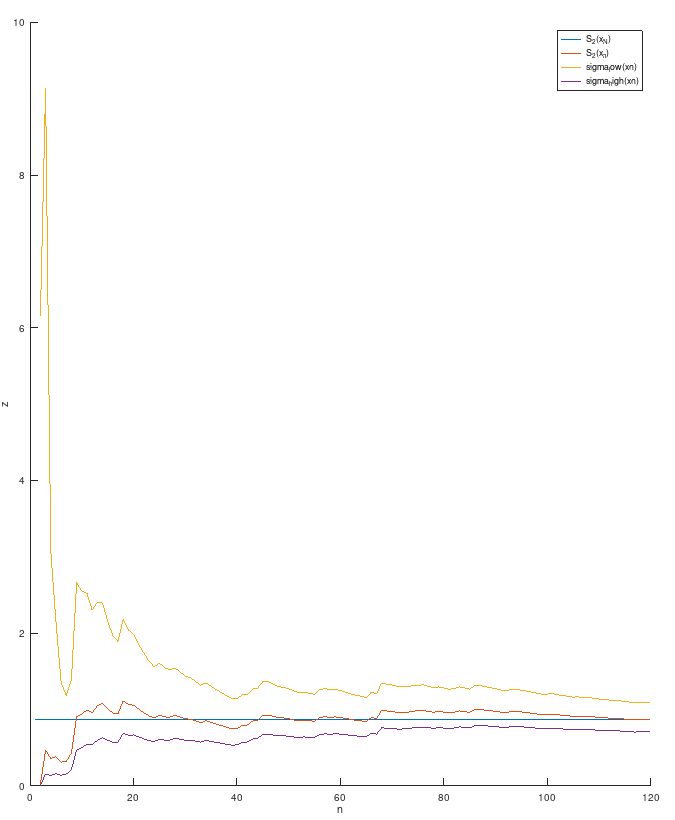
\includegraphics[scale=0.5]{./images/graph_2}
		\caption{График прямой $z=S^2(\vec x_N)$ и функций $z=S^2(\vec x_n), \newline z=\underline\sigma^2(\vec x_n),\  z=\overline\sigma^2(\vec x_n)$ как функции объема n выборки, где n изменяется от 1 до N.}
		\label{image:graph2}
	}
\end{figure}